% !TEX encoding = UTF-8 Unicode

\documentclass{standalone}

% packages
\usepackage{float}
\usepackage{tabu}
\usepackage{booktabs}
\usepackage{graphicx}
\usepackage{caption}
\usepackage[export]{adjustbox}
\usepackage[utf8]{inputenc}
%\usepackage[active,pdftex,tightpage]{preview}
\usepackage{newtxtext,newtxmath}

\begin{document}

%\sf
\scriptsize
\centering 

\begin{tabular}{m{0.5\textwidth} m{0.5\textwidth}}
%
\multicolumn{1}{c}{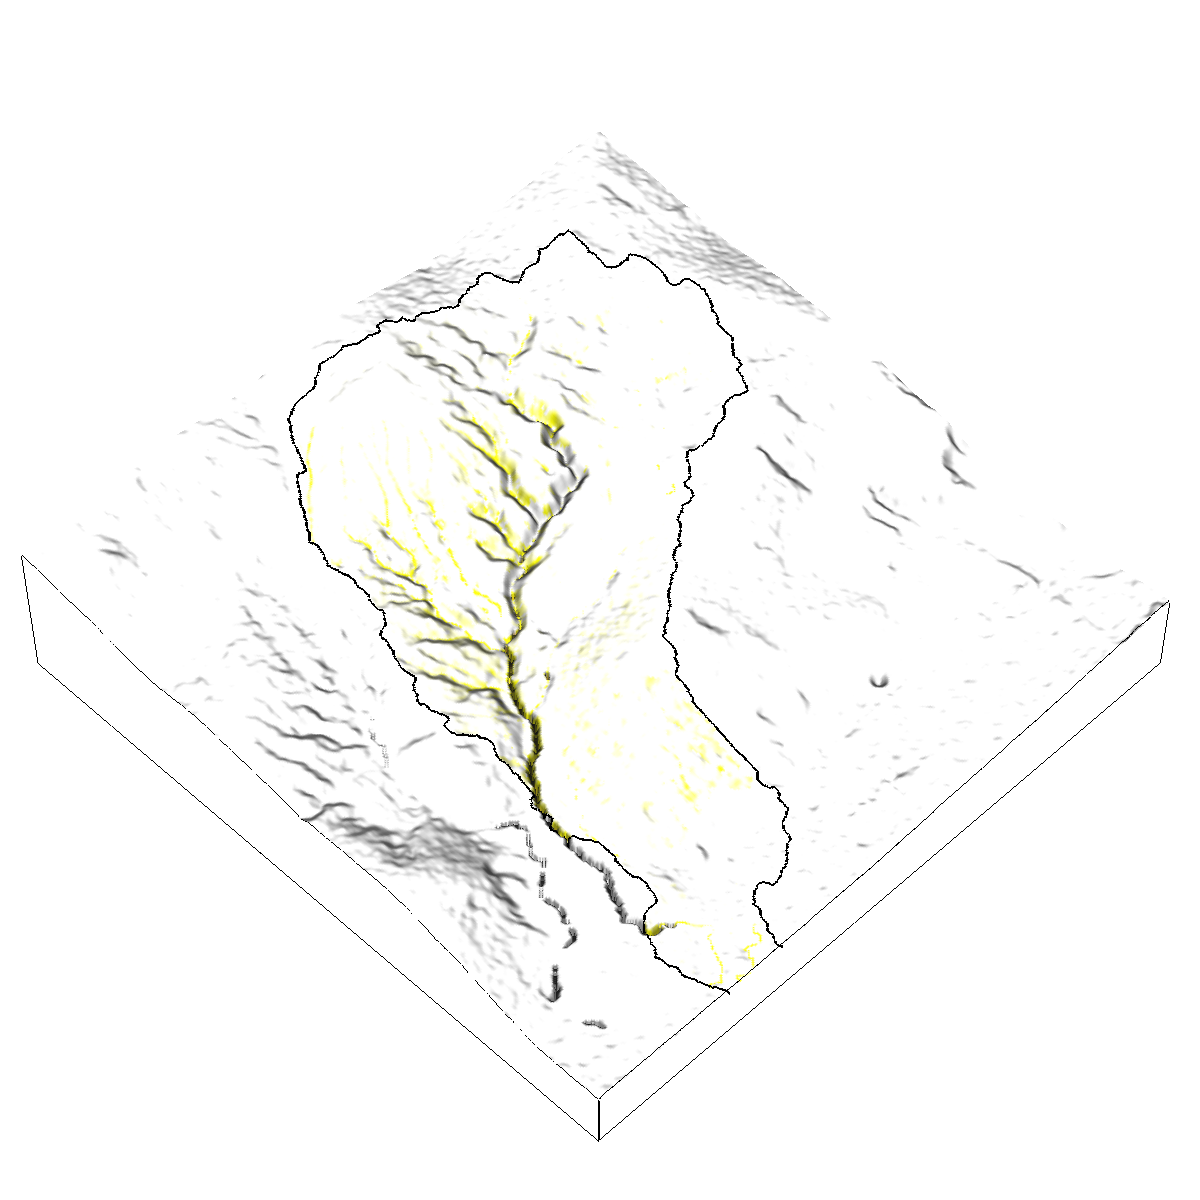
\includegraphics[height=50mm]{../../images/rusle_3d/flux.png}} &
\multicolumn{1}{c}{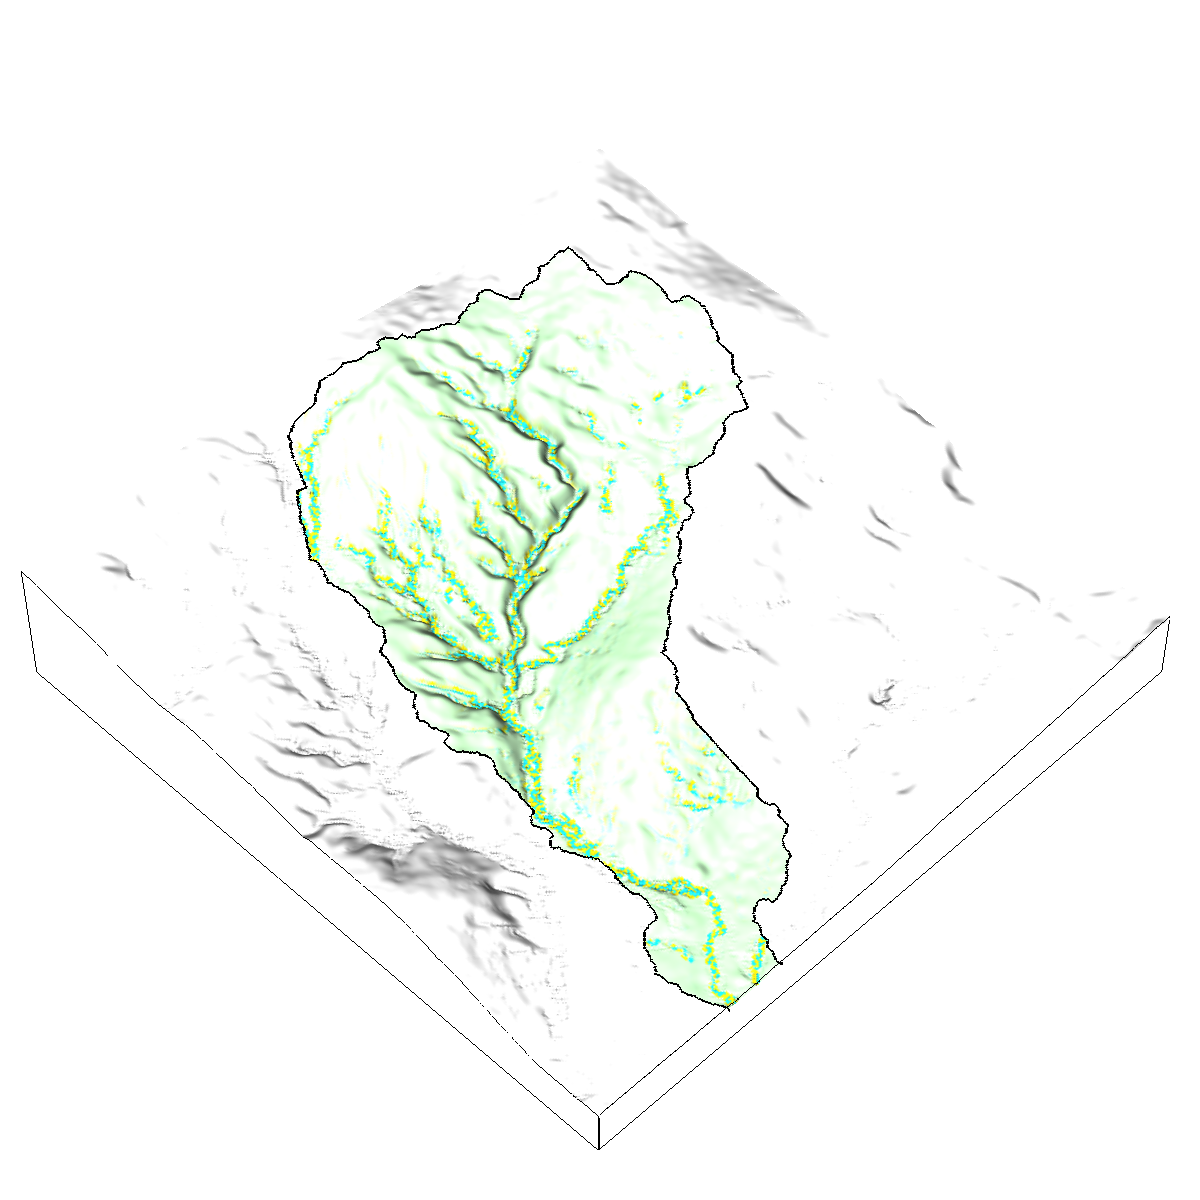
\includegraphics[height=50mm]{../../images/usped_3d/erosion_deposition.png}}\\
\multicolumn{1}{c}{a. Dynamic RUSLE3D sediment flow $(kg ~ m^{-2} ~ s^{-1})$} &
\multicolumn{1}{c}{d. Dynamic USPED erosion-deposition $(kg ~ m^{-2} ~ s^{-1})$}\\
%
\multicolumn{1}{c}{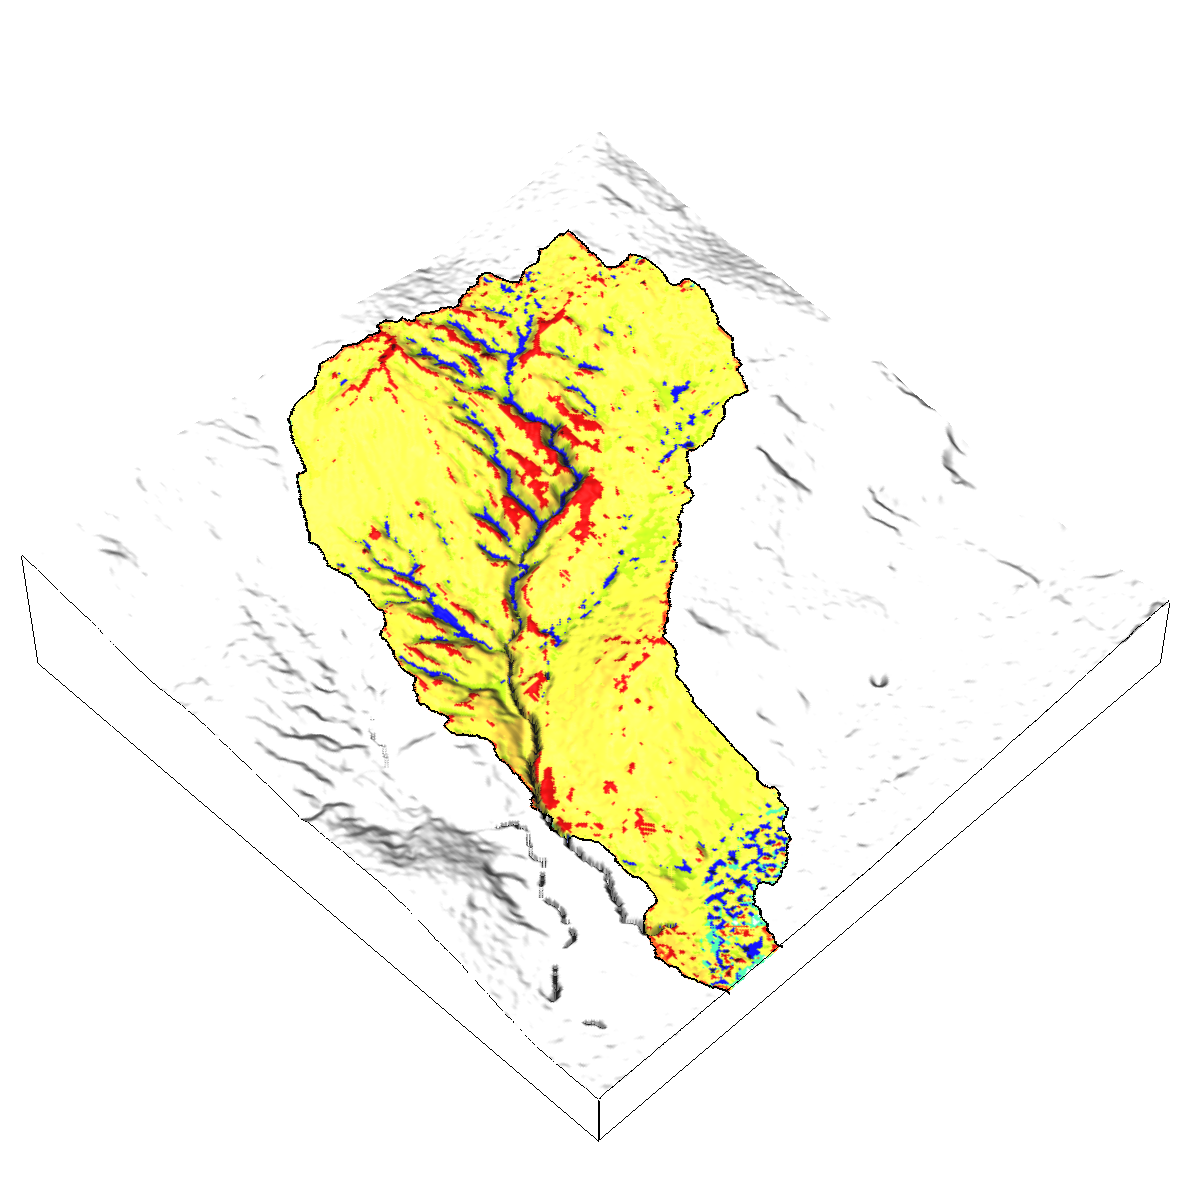
\includegraphics[height=50mm]{../../images/rusle_3d/landforms.png}} &
\multicolumn{1}{c}{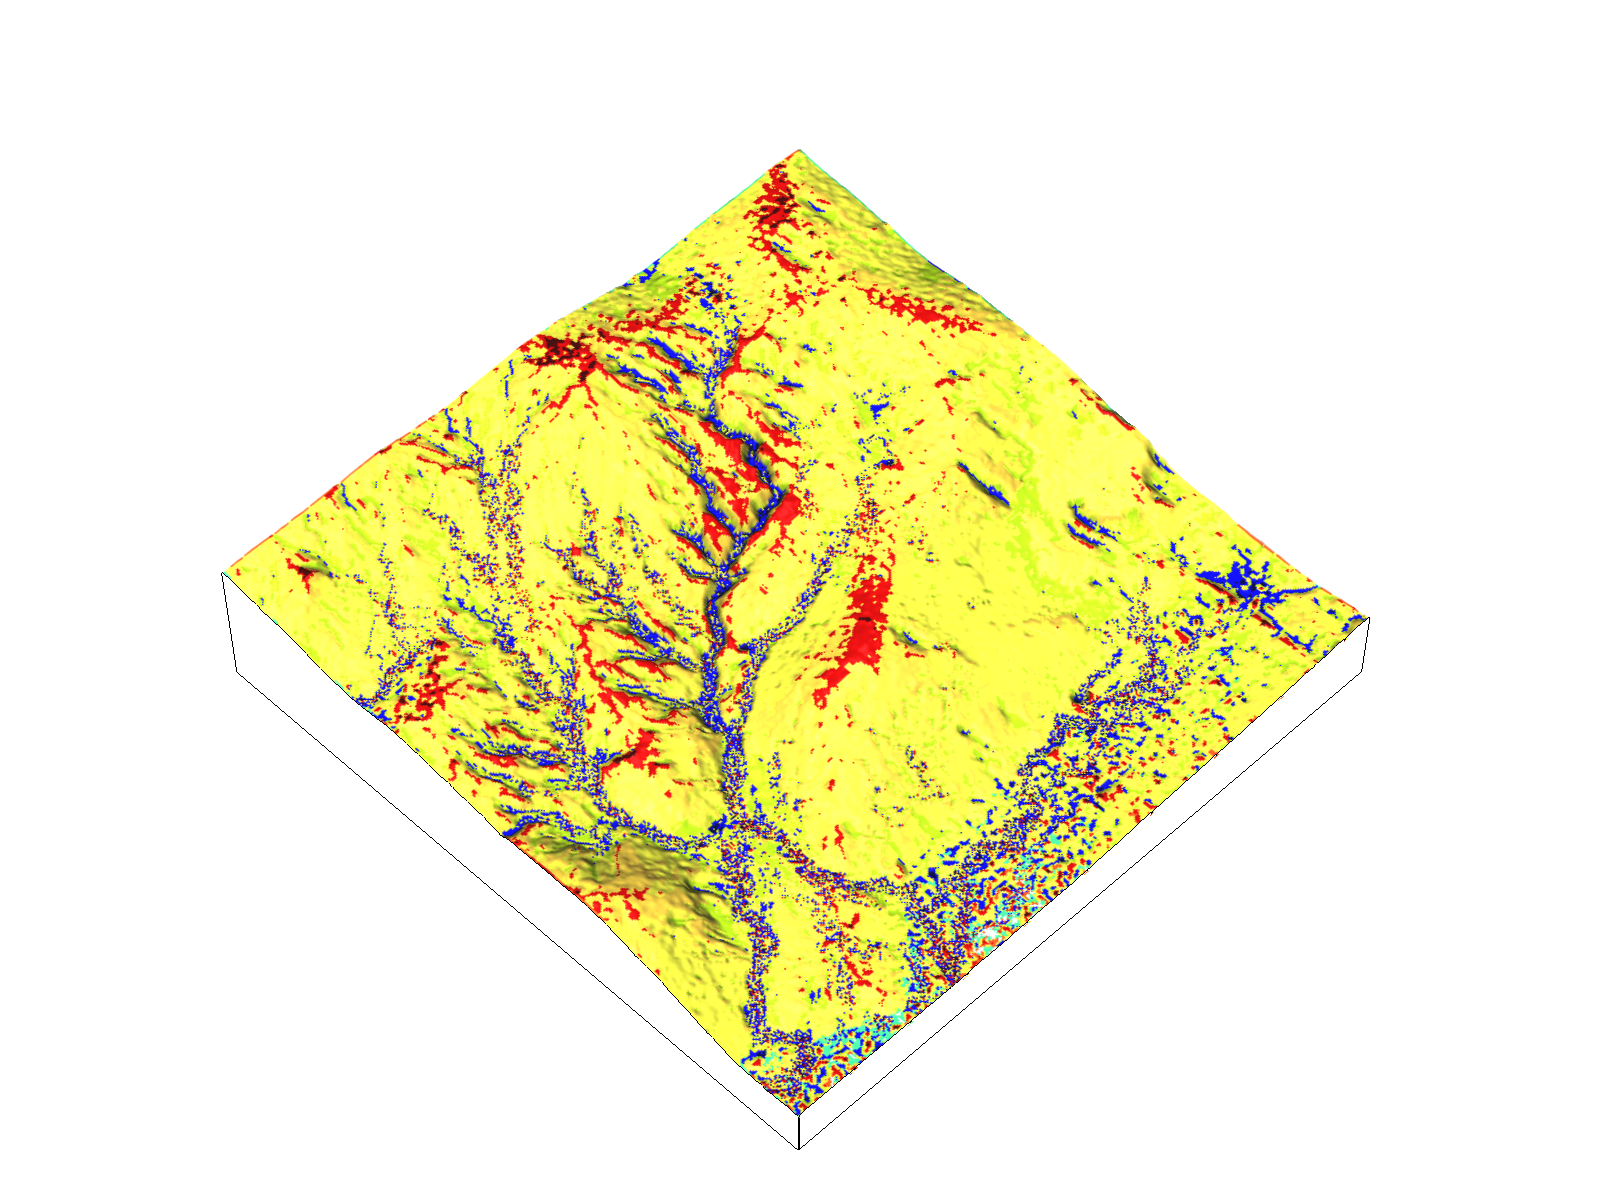
\includegraphics[height=50mm]{../../images/usped_3d/landforms.png}}\\
\multicolumn{1}{c}{b. Dynamic RUSLE3D landforms} &
\multicolumn{1}{c}{e. Dynamic USPED landforms}\\
%
\multicolumn{1}{c}{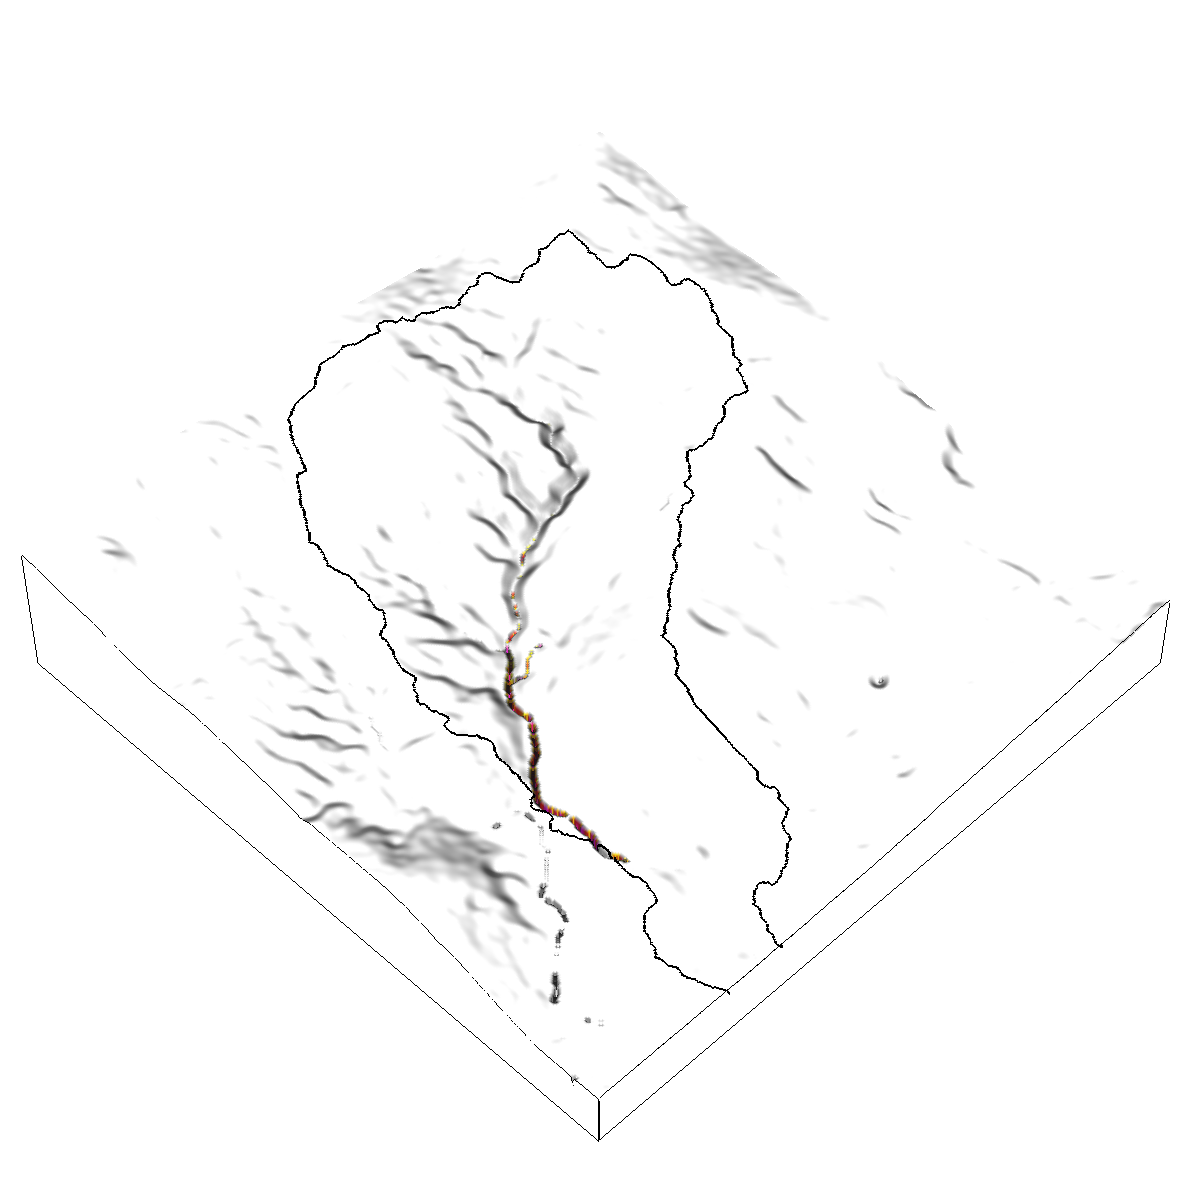
\includegraphics[height=50mm]{../../images/rusle_3d/difference.png}} &
\multicolumn{1}{c}{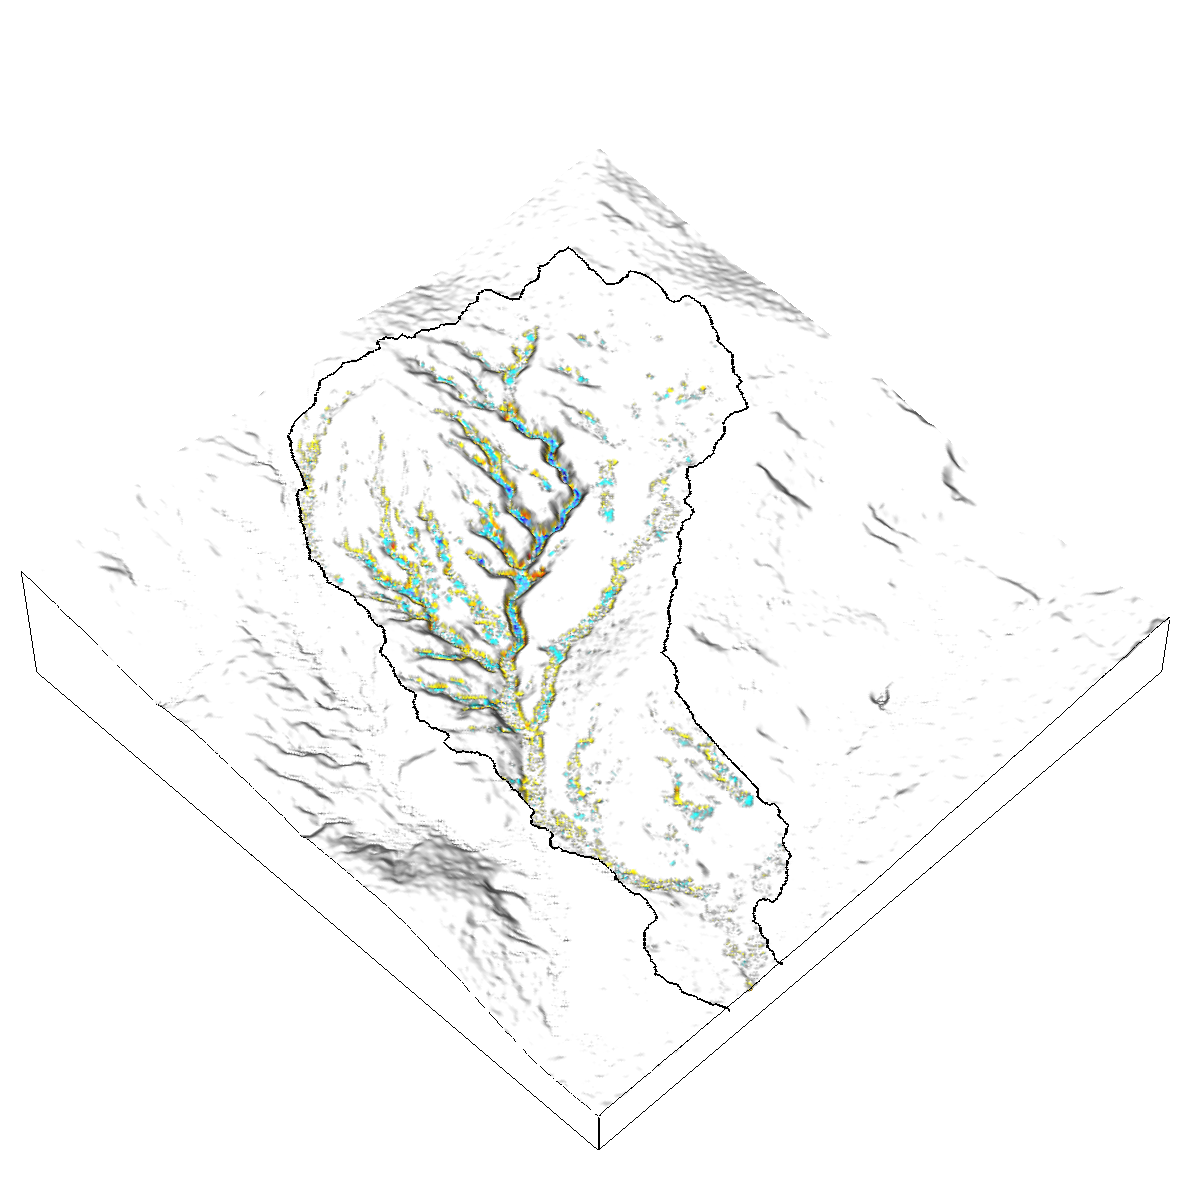
\includegraphics[height=50mm]{../../images/usped_3d/difference.png}}\\
\multicolumn{1}{c}{c. Dynamic RUSLE3D net difference $(m)$} & 
\multicolumn{1}{c}{f. Dynamic USPED net difference $(m)$}\\

%
\end{tabular}

% add legend

\end{document}